\subsection{Part I}

Since the arrival rate and the number of stations is fixed, and the probability
of error varies, in order to select a scheme among the three queueing systems,
it is reasonable to consider the metric of end-to-end delay as the decisive
factor. The system that exhibits the least average delay is the one we shall
choose as the most preferable.

Figure \ref{fig:06_delay_1} shows the relation between the end-to-end delay
and the probability of error $p_{e,i}$, $i = \{1,2, \dots r+1\}$ for the three
different queueing networks considered.

\begin{figure}[H]\centering
  % This file was created by matlab2tikz.
%
%The latest updates can be retrieved from
%  http://www.mathworks.com/matlabcentral/fileexchange/22022-matlab2tikz-matlab2tikz
%where you can also make suggestions and rate matlab2tikz.
%
\definecolor{mycolor1}{rgb}{0.00000,0.44700,0.74100}%
\definecolor{mycolor2}{rgb}{0.85000,0.32500,0.09800}%
\definecolor{mycolor3}{rgb}{0.92900,0.69400,0.12500}%
%
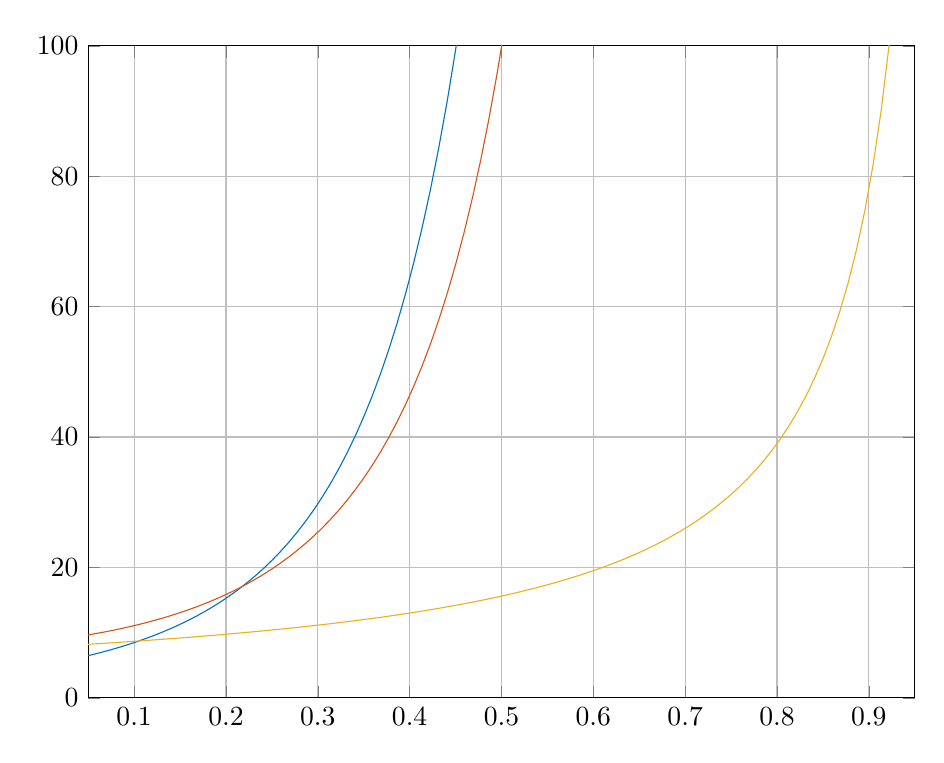
\begin{tikzpicture}

\begin{axis}[%
width=4.133in,
height=3.26in,
at={(0.693in,0.44in)},
scale only axis,
xmin=0.05,
xmax=0.95,
xmajorgrids,
ymin=0,
ymax=100,
ymajorgrids,
axis background/.style={fill=white}
]
\addplot [color=mycolor1,solid,forget plot]
  table[row sep=crcr]{%
0.05	6.46177717449908\\
0.0590909090909091	6.78003102478661\\
0.0681818181818182	7.11728084369001\\
0.0772727272727273	7.47486268334518\\
0.0863636363636364	7.85422107549834\\
0.0954545454545455	8.25691904165264\\
0.104545454545455	8.68464914014728\\
0.113636363636364	9.13924566955701\\
0.122727272727273	9.62269816295295\\
0.131818181818182	10.1371663248255\\
0.140909090909091	10.6849965821531\\
0.15	11.2687404435799\\
0.159090909090909	11.8911748863711\\
0.168181818181818	12.5553250202535\\
0.177272727272727	13.2644893110062\\
0.186363636363636	14.0222676854426\\
0.195454545454545	14.8325928840178\\
0.204545454545455	15.6997654786696\\
0.213636363636364	16.628493032774\\
0.222727272727273	17.6239339485893\\
0.231818181818182	18.6917466268415\\
0.240909090909091	19.8381446550243\\
0.25	21.0699588477366\\
0.259090909090909	22.3947070865765\\
0.268181818181818	23.8206730518608\\
0.277272727272727	25.3569951074505\\
0.286363636363636	27.0137667976755\\
0.295454545454545	28.80215064708\\
0.304545454545455	30.734507225846\\
0.313636363636364	32.8245417639804\\
0.322727272727273	35.0874709749517\\
0.331818181818182	37.540213195666\\
0.340909090909091	40.2016054780744\\
0.35	43.0926518948647\\
0.359090909090909	46.2368080677634\\
0.368181818181818	49.6603078165982\\
0.377272727272727	53.3925388906457\\
0.386363636363636	57.4664760179991\\
0.395454545454545	61.9191810394628\\
0.404545454545454	66.792381737305\\
0.413636363636364	72.1331431961281\\
0.422727272727273	77.9946482302495\\
0.431818181818182	84.437106688\\
0.440909090909091	91.5288174342852\\
0.45	99.3474116894648\\
0.459090909090909	107.981312380495\\
0.468181818181818	117.531451511793\\
0.477272727272727	128.11329663444\\
0.486363636363636	139.859248724235\\
0.495454545454545	152.921487736254\\
0.504545454545455	167.475359511576\\
0.513636363636364	183.723419507239\\
0.522727272727273	201.900276217459\\
0.531818181818182	222.278411734166\\
0.540909090909091	245.175200727607\\
0.55	270.961404934884\\
0.559090909090909	300.071491623905\\
0.568181818181818	333.016216233681\\
0.577272727272727	370.398027868827\\
0.586363636363636	412.930010133864\\
0.595454545454545	461.459270542232\\
0.604545454545454	516.99595522215\\
0.613636363636364	580.749413497275\\
0.622727272727273	654.173498965849\\
0.631818181818182	739.023611342582\\
0.640909090909091	837.4289144773\\
0.65	951.984292259177\\
0.659090909090909	1085.86814156379\\
0.668181818181818	1242.99421626391\\
0.677272727272727	1428.20866902082\\
0.686363636363636	1647.54753902314\\
0.695454545454545	1908.5757213461\\
0.704545454545455	2220.83669770236\\
0.713636363636364	2596.4541694632\\
0.722727272727273	3050.94397992159\\
0.731818181818182	3604.32007081634\\
0.740909090909091	4282.6159495072\\
0.75	5120\\
%0.759090909090909	6161.74981111046\\
%0.768181818181818	7468.48525588059\\
%0.777272727272727	9122.27180654686\\
%0.786363636363636	11235.5443604665\\
%0.795454545454546	13964.3536723738\\
%0.804545454545454	17528.3537966591\\
%0.813636363636364	22241.5026365313\\
%0.822727272727273	28560.1427173656\\
%0.831818181818182	37159.9215199098\\
%0.840909090909091	49061.7671208426\\
%0.85	65843.6213991769\\
%0.859090909090909	90006.720772125\\
%0.868181818181818	125630.017118982\\
%0.877272727272727	179582.737556247\\
%0.886363636363636	263865.9584\\
%0.895454545454545	400354.051982623\\
%0.904545454545455	630938.363179559\\
%0.913636363636364	1040675.67573025\\
%0.922727272727273	1814841.91717898\\
%0.931818181818182	3393337.94238685\\
%0.940909090909091	6940114.68031979\\
%0.95	15999999.9999999\\
};
\addplot [color=mycolor2,solid,forget plot]
  table[row sep=crcr]{%
0.05	9.64907000294705\\
0.0590909090909091	9.87204156299107\\
0.0681818181818182	10.1099680285732\\
0.0772727272727273	10.3635230072907\\
0.0863636363636364	10.6334553029567\\
0.0954545454545455	10.9205926071121\\
0.104545454545455	11.2258459659832\\
0.113636363636364	11.5502150425106\\
0.122727272727273	11.894794207916\\
0.131818181818182	12.260779511589\\
0.140909090909091	12.6494765923485\\
0.15	13.0623096088148\\
0.159090909090909	13.5008312821033\\
0.168181818181818	13.966734160722\\
0.177272727272727	14.4618632358085\\
0.186363636363636	14.9882300550919\\
0.195454545454545	15.5480285066676\\
0.204545454545455	16.1436524693128\\
0.213636363636364	16.7777155552285\\
0.222727272727273	17.4530732044036\\
0.231818181818182	18.1728474280132\\
0.240909090909091	18.9404545422637\\
0.25	19.7596362849042\\
0.259090909090909	20.6344947654508\\
0.268181818181818	21.5695317684554\\
0.277272727272727	22.5696930085904\\
0.286363636363636	23.6404180289578\\
0.295454545454545	24.7876965422778\\
0.304545454545455	26.0181321413903\\
0.313636363636364	27.3390144542921\\
0.322727272727273	28.7584009939415\\
0.331818181818182	30.2852101593659\\
0.340909090909091	31.929327088345\\
0.35	33.7017243505566\\
0.359090909090909	35.6145998126435\\
0.368181818181818	37.6815344142129\\
0.377272727272727	39.9176730798694\\
0.386363636363636	42.339932573551\\
0.395454545454545	44.9672407981225\\
0.404545454545454	47.8208128805073\\
0.413636363636364	50.924470391782\\
0.422727272727273	54.3050112712538\\
0.431818181818182	57.9926395017502\\
0.440909090909091	62.0214653803322\\
0.45	66.4300894198379\\
0.459090909090909	71.2622855969971\\
0.468181818181818	76.5678029522191\\
0.477272727272727	82.4033085965139\\
0.486363636363636	88.8335001857793\\
0.495454545454545	95.9324221289847\\
0.504545454545455	103.785027521692\\
0.513636363636364	112.489037448448\\
0.522727272727273	122.157161405667\\
0.531818181818182	132.919757848336\\
0.540909090909091	144.928033157546\\
0.55	158.357901841012\\
0.559090909090909	173.414662071982\\
0.568181818181818	190.338680808481\\
0.577272727272727	209.412334469912\\
0.586363636363636	230.968518178552\\
0.595454545454545	255.401123889913\\
0.604545454545454	283.178002116332\\
0.613636363636364	314.857072659718\\
0.622727272727273	351.106449566966\\
0.631818181818182	392.729712086892\\
0.640909090909091	440.697811432245\\
0.65	496.189587384854\\
0.659090909090909	560.643528529533\\
0.668181818181818	635.82431571218\\
0.677272727272727	723.908942044029\\
0.686363636363636	827.598952854983\\
0.695454545454545	950.267813907255\\
0.704545454545455	1096.15592083202\\
0.713636363636364	1270.63079570565\\
0.722727272727273	1480.53732114302\\
0.731818181818182	1734.67358282427\\
0.740909090909091	2044.44381384022\\
%0.75	2424.76388398664\\
%0.759090909090909	2895.33129058608\\
%0.768181818181818	3482.42808406281\\
%0.777272727272727	4221.51387612461\\
%0.786363636363636	5161.00776475935\\
%0.795454545454546	6367.88837785193\\
%0.804545454545454	7936.12309080682\\
%0.813636363636364	9999.58380451935\\
%0.822727272727273	12752.2258227411\\
%0.831818181818182	16480.2929405995\\
%0.840909090909091	21614.9354329875\\
%0.85	28820.4382445936\\
%0.859090909090909	39146.4892697244\\
%0.868181818181818	54299.5954103659\\
%0.877272727272727	77144.8128283093\\
%0.886363636363636	112672.396862104\\
%0.895454545454545	169950.663491739\\
%0.904545454545455	266294.295355689\\
%0.913636363636364	436754.94336275\\
%0.922727272727273	757459.315071054\\
%0.931818181818182	1408625.91633851\\
%0.940909090909091	2865712.45818029\\
%0.95	6572522.60163537\\
};
\addplot [color=mycolor3,solid,forget plot]
  table[row sep=crcr]{%
0.05	8.21052631578947\\
0.0590909090909091	8.28985507246377\\
0.0681818181818182	8.37073170731707\\
0.0772727272727273	8.45320197044335\\
0.0863636363636364	8.53731343283582\\
0.0954545454545455	8.62311557788945\\
0.104545454545455	8.71065989847716\\
0.113636363636364	8.8\\
0.122727272727273	8.89119170984456\\
0.131818181818182	8.98429319371728\\
0.140909090909091	9.07936507936508\\
0.15	9.17647058823529\\
0.159090909090909	9.27567567567568\\
0.168181818181818	9.37704918032787\\
0.177272727272727	9.48066298342541\\
0.186363636363636	9.58659217877095\\
0.195454545454545	9.69491525423729\\
0.204545454545455	9.80571428571429\\
0.213636363636364	9.91907514450867\\
0.222727272727273	10.0350877192982\\
0.231818181818182	10.1538461538462\\
0.240909090909091	10.2754491017964\\
0.25	10.4\\
0.259090909090909	10.5276073619632\\
0.268181818181818	10.6583850931677\\
0.277272727272727	10.7924528301887\\
0.286363636363636	10.9299363057325\\
0.295454545454545	11.0709677419355\\
0.304545454545455	11.2156862745098\\
0.313636363636364	11.364238410596\\
0.322727272727273	11.5167785234899\\
0.331818181818182	11.6734693877551\\
0.340909090909091	11.8344827586207\\
0.35	12\\
0.359090909090909	12.1702127659574\\
0.368181818181818	12.3453237410072\\
0.377272727272727	12.5255474452555\\
0.386363636363636	12.7111111111111\\
0.395454545454545	12.9022556390977\\
0.404545454545454	13.0992366412214\\
0.413636363636364	13.3023255813953\\
0.422727272727273	13.511811023622\\
0.431818181818182	13.728\\
0.440909090909091	13.9512195121951\\
0.45	14.1818181818182\\
0.459090909090909	14.4201680672269\\
0.468181818181818	14.6666666666667\\
0.477272727272727	14.9217391304348\\
0.486363636363636	15.1858407079646\\
0.495454545454545	15.4594594594595\\
0.504545454545455	15.743119266055\\
0.513636363636364	16.0373831775701\\
0.522727272727273	16.3428571428571\\
0.531818181818182	16.6601941747573\\
0.540909090909091	16.990099009901\\
0.55	17.3333333333333\\
0.559090909090909	17.6907216494845\\
0.568181818181818	18.0631578947368\\
0.577272727272727	18.4516129032258\\
0.586363636363636	18.8571428571429\\
0.595454545454545	19.2808988764045\\
0.604545454545454	19.7241379310345\\
0.613636363636364	20.1882352941176\\
0.622727272727273	20.6746987951807\\
0.631818181818182	21.1851851851852\\
0.640909090909091	21.7215189873418\\
0.65	22.2857142857143\\
0.659090909090909	22.88\\
0.668181818181818	23.5068493150685\\
0.677272727272727	24.169014084507\\
0.686363636363636	24.8695652173913\\
0.695454545454545	25.6119402985075\\
0.704545454545455	26.4\\
0.713636363636364	27.2380952380952\\
0.722727272727273	28.1311475409836\\
0.731818181818182	29.0847457627119\\
0.740909090909091	30.1052631578947\\
0.75	31.2\\
0.759090909090909	32.377358490566\\
0.768181818181818	33.6470588235294\\
0.777272727272727	35.0204081632653\\
0.786363636363636	36.5106382978723\\
0.795454545454546	38.1333333333333\\
0.804545454545454	39.906976744186\\
0.813636363636364	41.8536585365854\\
0.822727272727273	44\\
0.831818181818182	46.3783783783784\\
0.840909090909091	49.0285714285714\\
0.85	52\\
0.859090909090909	55.3548387096774\\
0.868181818181818	59.1724137931034\\
0.877272727272727	63.5555555555555\\
0.886363636363636	68.64\\
0.895454545454545	74.6086956521739\\
0.904545454545455	81.7142857142857\\
0.913636363636364	90.3157894736841\\
0.922727272727273	100.941176470588\\
0.931818181818182	114.4\\
0.940909090909091	132\\
0.95	156\\
};
\end{axis}
\end{tikzpicture}%

  \caption{The relation between end-to-end delay and the probability of error
    in a queueing network with AF relaying with end-to-end AQR (\texttt{blue}),
    DF relaying and end-to-end ARQ (\texttt{red}) and
    DF relaying and hop-by-hop ARQ (\texttt{orange}) for $r=4$.}
  \label{fig:06_delay_1}
\end{figure}

What is evident here is that as the probability of error increases, the average
delay in the AF relaying with hop-by-hop ARQ system increases in a less rapid
fashion compared to the other two queueing networks. This system can tolerate
larger probability errors, and hence be more robust, while at the same time
appear lower end-to-end delay times.


% ------------------------------------------------------------------------------
\subsection{Part II}

Since the arrival rate, the number of stations, and the probability of error is
fixed, in order to select a scheme among the three queueing systems,
it is reasonable to consider the metric of end-to-end delay as the decisive
factor. The system that exhibits the least average delay is the one we shall
choose as the most preferable.

Figure \ref{fig:06_delay_2} shows the relation between the end-to-end delay
and the value of $k \in [1,4]$ for the three different queueing networks
considered.

Consulting figure \ref{fig:06_delay_3}, which shows a magnified portion of this
relation, it is evident that for $k \in [1, 1.97]$, DF relaying with hop-by-hop
ARQ exhibits lower average delay times than the other two queueing systems,
while for $k \in [1.97, 4]$ the lowest average delay times are exhibited by
the AF relaying with end-to-end ARQ system.

\begin{figure}[H]\centering
  % This file was created by matlab2tikz.
%
%The latest updates can be retrieved from
%  http://www.mathworks.com/matlabcentral/fileexchange/22022-matlab2tikz-matlab2tikz
%where you can also make suggestions and rate matlab2tikz.
%
\definecolor{mycolor1}{rgb}{0.00000,0.44700,0.74100}%
\definecolor{mycolor2}{rgb}{0.85000,0.32500,0.09800}%
\definecolor{mycolor3}{rgb}{0.92900,0.69400,0.12500}%
%
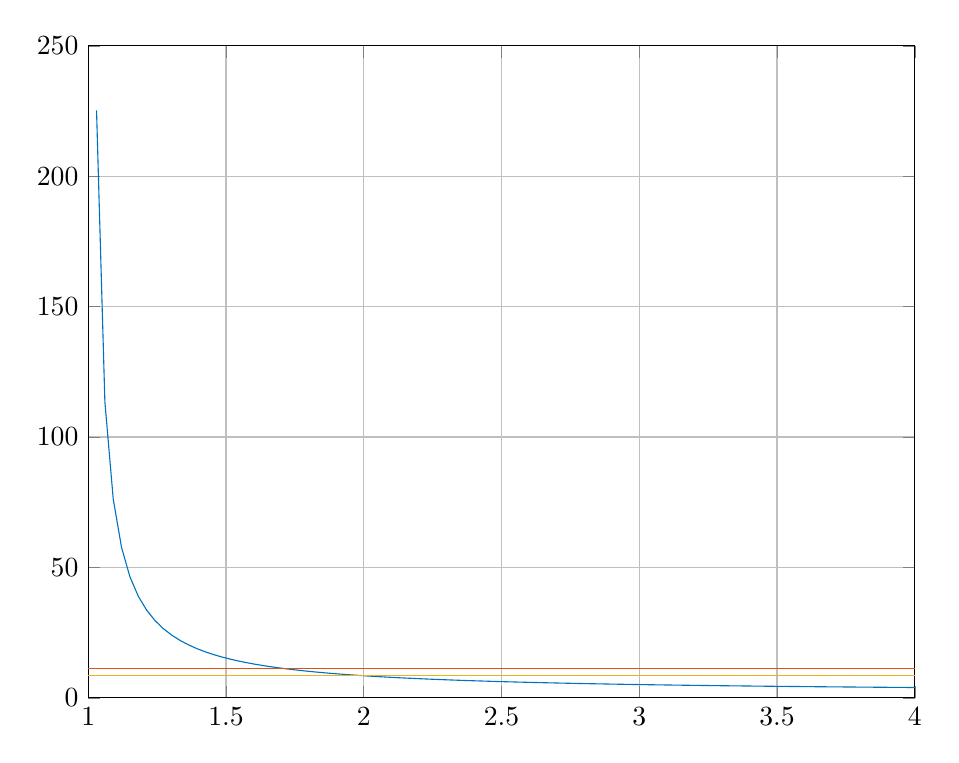
\begin{tikzpicture}

\begin{axis}[%
width=4.133in,
height=3.26in,
at={(0.693in,0.44in)},
scale only axis,
unbounded coords=jump,
xmin=1,
xmax=4,
xmajorgrids,
ymin=0,
ymax=250,
ymajorgrids,
axis background/.style={fill=white}
]
\addplot [color=mycolor1,solid,forget plot]
  table[row sep=crcr]{%
1	inf\\
1.03030303030303	225.236667852122\\
1.06060606060606	113.465088316483\\
1.09090909090909	76.2078951379363\\
1.12121212121212	57.579298548663\\
1.15151515151515	46.402140595099\\
1.18181818181818	38.9507019593896\\
1.21212121212121	33.6282457910258\\
1.24242424242424	29.636403664753\\
1.27272727272727	26.5316375665408\\
1.3030303030303	24.047824687971\\
1.33333333333333	22.0156141509594\\
1.36363636363636	20.3221053701163\\
1.39393939393939	18.8891364017107\\
1.42424242424242	17.6608772859344\\
1.45454545454545	16.5963860522617\\
1.48484848484848	15.664956222798\\
1.51515151515152	14.8431063732713\\
1.54545454545455	14.1125731736919\\
1.57575757575758	13.4589382056472\\
1.60606060606061	12.870666734407\\
1.63636363636364	12.3384211175706\\
1.66666666666667	11.8545614659012\\
1.6969696969697	11.4127765665508\\
1.72727272727273	11.0078070754797\\
1.75757575757576	10.6352351436942\\
1.78787878787879	10.2913225912769\\
1.81818181818182	9.97288504274228\\
1.84848484848485	9.67719303338873\\
1.87878787878788	9.4018935764044\\
1.90909090909091	9.14494741655235\\
1.93939393939394	8.90457842830367\\
1.96969696969697	8.67923250182052\\
2	8.46754390421514\\
2.03030303030303	8.26830757705714\\
2.06060606060606	8.08045618287959\\
2.09090909090909	7.90304097726747\\
2.12121212121212	7.73521578276951\\
2.15151515151515	7.57622349324513\\
2.18181818181818	7.42538465446559\\
2.21212121212121	7.28208775762502\\
2.24242424242424	7.14578095331327\\
2.27272727272727	7.01596494920683\\
2.3030303030303	6.89218689877977\\
2.33333333333333	6.77403512337212\\
2.36363636363636	6.66113453798258\\
2.39393939393939	6.55314267369694\\
2.42424242424242	6.44974620789153\\
2.45454545454545	6.35065792816136\\
2.48484848484848	6.255614068012\\
2.51515151515152	6.16437196226862\\
2.54545454545455	6.0767079783191\\
2.57575757575758	5.99241568605995\\
2.60606060606061	5.91130423501812\\
2.63636363636364	5.83319691179265\\
2.66666666666667	5.7579298548663\\
2.6969696969697	5.68535090711588\\
2.72727272727273	5.61531858911109\\
2.75757575757576	5.54770117862371\\
2.78787878787879	5.48237588374607\\
2.81818181818182	5.41922809869769\\
2.84848484848485	5.35815073283122\\
2.87878787878788	5.29904360457335\\
2.90909090909091	5.24181289308556\\
2.93939393939394	5.18637064133177\\
2.96969696969697	5.13263430501656\\
3	5.08052634252908\\
3.03030303030303	5.0299738416084\\
3.06060606060606	4.98090817895008\\
3.09090909090909	4.9332647094123\\
3.12121212121212	4.88698248186131\\
3.15151515151515	4.84200397903007\\
3.18181818181818	4.79827487905525\\
3.21212121212121	4.75574383661398\\
3.24242424242424	4.71436228180627\\
3.27272727272727	4.67408423512676\\
3.3030303030303	4.63486613704408\\
3.33333333333333	4.59666669085965\\
3.36363636363636	4.55944671765431\\
3.39393939393939	4.52316902225163\\
3.42424242424242	4.48779826923403\\
3.45454545454545	4.45330086814278\\
3.48484848484848	4.41964486707815\\
3.51515151515152	4.38679985399098\\
3.54545454545455	4.35473686502493\\
3.57575757575758	4.32342829932867\\
3.60606060606061	4.2928478398114\\
3.63636363636364	4.26297037936349\\
3.66666666666667	4.23377195210757\\
3.6969696969697	4.20522966928437\\
3.72727272727273	4.1773216594128\\
3.75757575757576	4.15002701239555\\
3.78787878787879	4.12332572726998\\
3.81818181818182	4.09719866332991\\
3.84848484848485	4.07162749436728\\
3.87878787878788	4.04659466580387\\
3.90909090909091	4.02208335450219\\
3.93939393939394	3.99807743106241\\
3.96969696969697	3.97456142442752\\
4	3.95152048863373\\
};
\addplot [color=mycolor2,solid,forget plot]
  table[row sep=crcr]{%
1	11.0708944449598\\
1.03030303030303	11.0708944449598\\
1.06060606060606	11.0708944449598\\
1.09090909090909	11.0708944449598\\
1.12121212121212	11.0708944449598\\
1.15151515151515	11.0708944449598\\
1.18181818181818	11.0708944449598\\
1.21212121212121	11.0708944449598\\
1.24242424242424	11.0708944449598\\
1.27272727272727	11.0708944449598\\
1.3030303030303	11.0708944449598\\
1.33333333333333	11.0708944449598\\
1.36363636363636	11.0708944449598\\
1.39393939393939	11.0708944449598\\
1.42424242424242	11.0708944449598\\
1.45454545454545	11.0708944449598\\
1.48484848484848	11.0708944449598\\
1.51515151515152	11.0708944449598\\
1.54545454545455	11.0708944449598\\
1.57575757575758	11.0708944449598\\
1.60606060606061	11.0708944449598\\
1.63636363636364	11.0708944449598\\
1.66666666666667	11.0708944449598\\
1.6969696969697	11.0708944449598\\
1.72727272727273	11.0708944449598\\
1.75757575757576	11.0708944449598\\
1.78787878787879	11.0708944449598\\
1.81818181818182	11.0708944449598\\
1.84848484848485	11.0708944449598\\
1.87878787878788	11.0708944449598\\
1.90909090909091	11.0708944449598\\
1.93939393939394	11.0708944449598\\
1.96969696969697	11.0708944449598\\
2	11.0708944449598\\
2.03030303030303	11.0708944449598\\
2.06060606060606	11.0708944449598\\
2.09090909090909	11.0708944449598\\
2.12121212121212	11.0708944449598\\
2.15151515151515	11.0708944449598\\
2.18181818181818	11.0708944449598\\
2.21212121212121	11.0708944449598\\
2.24242424242424	11.0708944449598\\
2.27272727272727	11.0708944449598\\
2.3030303030303	11.0708944449598\\
2.33333333333333	11.0708944449598\\
2.36363636363636	11.0708944449598\\
2.39393939393939	11.0708944449598\\
2.42424242424242	11.0708944449598\\
2.45454545454545	11.0708944449598\\
2.48484848484848	11.0708944449598\\
2.51515151515152	11.0708944449598\\
2.54545454545455	11.0708944449598\\
2.57575757575758	11.0708944449598\\
2.60606060606061	11.0708944449598\\
2.63636363636364	11.0708944449598\\
2.66666666666667	11.0708944449598\\
2.6969696969697	11.0708944449598\\
2.72727272727273	11.0708944449598\\
2.75757575757576	11.0708944449598\\
2.78787878787879	11.0708944449598\\
2.81818181818182	11.0708944449598\\
2.84848484848485	11.0708944449598\\
2.87878787878788	11.0708944449598\\
2.90909090909091	11.0708944449598\\
2.93939393939394	11.0708944449598\\
2.96969696969697	11.0708944449598\\
3	11.0708944449598\\
3.03030303030303	11.0708944449598\\
3.06060606060606	11.0708944449598\\
3.09090909090909	11.0708944449598\\
3.12121212121212	11.0708944449598\\
3.15151515151515	11.0708944449598\\
3.18181818181818	11.0708944449598\\
3.21212121212121	11.0708944449598\\
3.24242424242424	11.0708944449598\\
3.27272727272727	11.0708944449598\\
3.3030303030303	11.0708944449598\\
3.33333333333333	11.0708944449598\\
3.36363636363636	11.0708944449598\\
3.39393939393939	11.0708944449598\\
3.42424242424242	11.0708944449598\\
3.45454545454545	11.0708944449598\\
3.48484848484848	11.0708944449598\\
3.51515151515152	11.0708944449598\\
3.54545454545455	11.0708944449598\\
3.57575757575758	11.0708944449598\\
3.60606060606061	11.0708944449598\\
3.63636363636364	11.0708944449598\\
3.66666666666667	11.0708944449598\\
3.6969696969697	11.0708944449598\\
3.72727272727273	11.0708944449598\\
3.75757575757576	11.0708944449598\\
3.78787878787879	11.0708944449598\\
3.81818181818182	11.0708944449598\\
3.84848484848485	11.0708944449598\\
3.87878787878788	11.0708944449598\\
3.90909090909091	11.0708944449598\\
3.93939393939394	11.0708944449598\\
3.96969696969697	11.0708944449598\\
4	11.0708944449598\\
};
\addplot [color=mycolor3,solid,forget plot]
  table[row sep=crcr]{%
1	8.66666666666667\\
1.03030303030303	8.66666666666667\\
1.06060606060606	8.66666666666667\\
1.09090909090909	8.66666666666667\\
1.12121212121212	8.66666666666667\\
1.15151515151515	8.66666666666667\\
1.18181818181818	8.66666666666667\\
1.21212121212121	8.66666666666667\\
1.24242424242424	8.66666666666667\\
1.27272727272727	8.66666666666667\\
1.3030303030303	8.66666666666667\\
1.33333333333333	8.66666666666667\\
1.36363636363636	8.66666666666667\\
1.39393939393939	8.66666666666667\\
1.42424242424242	8.66666666666667\\
1.45454545454545	8.66666666666667\\
1.48484848484848	8.66666666666667\\
1.51515151515152	8.66666666666667\\
1.54545454545455	8.66666666666667\\
1.57575757575758	8.66666666666667\\
1.60606060606061	8.66666666666667\\
1.63636363636364	8.66666666666667\\
1.66666666666667	8.66666666666667\\
1.6969696969697	8.66666666666667\\
1.72727272727273	8.66666666666667\\
1.75757575757576	8.66666666666667\\
1.78787878787879	8.66666666666667\\
1.81818181818182	8.66666666666667\\
1.84848484848485	8.66666666666667\\
1.87878787878788	8.66666666666667\\
1.90909090909091	8.66666666666667\\
1.93939393939394	8.66666666666667\\
1.96969696969697	8.66666666666667\\
2	8.66666666666667\\
2.03030303030303	8.66666666666667\\
2.06060606060606	8.66666666666667\\
2.09090909090909	8.66666666666667\\
2.12121212121212	8.66666666666667\\
2.15151515151515	8.66666666666667\\
2.18181818181818	8.66666666666667\\
2.21212121212121	8.66666666666667\\
2.24242424242424	8.66666666666667\\
2.27272727272727	8.66666666666667\\
2.3030303030303	8.66666666666667\\
2.33333333333333	8.66666666666667\\
2.36363636363636	8.66666666666667\\
2.39393939393939	8.66666666666667\\
2.42424242424242	8.66666666666667\\
2.45454545454545	8.66666666666667\\
2.48484848484848	8.66666666666667\\
2.51515151515152	8.66666666666667\\
2.54545454545455	8.66666666666667\\
2.57575757575758	8.66666666666667\\
2.60606060606061	8.66666666666667\\
2.63636363636364	8.66666666666667\\
2.66666666666667	8.66666666666667\\
2.6969696969697	8.66666666666667\\
2.72727272727273	8.66666666666667\\
2.75757575757576	8.66666666666667\\
2.78787878787879	8.66666666666667\\
2.81818181818182	8.66666666666667\\
2.84848484848485	8.66666666666667\\
2.87878787878788	8.66666666666667\\
2.90909090909091	8.66666666666667\\
2.93939393939394	8.66666666666667\\
2.96969696969697	8.66666666666667\\
3	8.66666666666667\\
3.03030303030303	8.66666666666667\\
3.06060606060606	8.66666666666667\\
3.09090909090909	8.66666666666667\\
3.12121212121212	8.66666666666667\\
3.15151515151515	8.66666666666667\\
3.18181818181818	8.66666666666667\\
3.21212121212121	8.66666666666667\\
3.24242424242424	8.66666666666667\\
3.27272727272727	8.66666666666667\\
3.3030303030303	8.66666666666667\\
3.33333333333333	8.66666666666667\\
3.36363636363636	8.66666666666667\\
3.39393939393939	8.66666666666667\\
3.42424242424242	8.66666666666667\\
3.45454545454545	8.66666666666667\\
3.48484848484848	8.66666666666667\\
3.51515151515152	8.66666666666667\\
3.54545454545455	8.66666666666667\\
3.57575757575758	8.66666666666667\\
3.60606060606061	8.66666666666667\\
3.63636363636364	8.66666666666667\\
3.66666666666667	8.66666666666667\\
3.6969696969697	8.66666666666667\\
3.72727272727273	8.66666666666667\\
3.75757575757576	8.66666666666667\\
3.78787878787879	8.66666666666667\\
3.81818181818182	8.66666666666667\\
3.84848484848485	8.66666666666667\\
3.87878787878788	8.66666666666667\\
3.90909090909091	8.66666666666667\\
3.93939393939394	8.66666666666667\\
3.96969696969697	8.66666666666667\\
4	8.66666666666667\\
};
\end{axis}
\end{tikzpicture}%
  \caption{The relation between end-to-end delay and $k \in [1,4]$
    in a queueing network with AF relaying with end-to-end AQR (\texttt{blue}),
    DF relaying and end-to-end ARQ (\texttt{red}) and
    DF relaying and hop-by-hop ARQ (\texttt{orange}) for $r=4$.}
  \label{fig:06_delay_2}
\end{figure}

\begin{figure}[H]\centering
  \input{./figures/af_or_df_2_magnified.tex}
  \caption{The relation between end-to-end delay and $k \in [1,4]$
    in a queueing network with AF relaying with end-to-end AQR (\texttt{blue}),
    DF relaying and end-to-end ARQ (\texttt{red}) and
    DF relaying and hop-by-hop ARQ (\texttt{orange}) for $r=4$,
    magnified to display the fine details of when the system exhibiting the
    lowest average delay changes.}
  \label{fig:06_delay_3}
\end{figure}
